%%%%%%%%%%%%%%%%%%%%%%%%%%%%%%%%%%%%%%%%%%%%%%%%%%%%%%%%%%%%%%%%%%%%%%%%%%%%%%%%
%2345678901234567890123456789012345678901234567890123456789012345678901234567890
%        1         2         3         4         5         6         7         8

\documentclass[letterpaper, 10 pt, conference]{ieeeconf}  % Comment this line out if you need a4paper

%\documentclass[a4paper, 10pt, conference]{ieeeconf}      % Use this line for a4 paper

\IEEEoverridecommandlockouts                              % This command is only needed if 
                                                          % you want to use the \thanks command

\overrideIEEEmargins                                      % Needed to meet printer requirements.

%In case you encounter the following error:
%Error 1010 The PDF file may be corrupt (unable to open PDF file) OR
%Error 1000 An error occurred while parsing a contents stream. Unable to analyze the PDF file.
%This is a known problem with pdfLaTeX conversion filter. The file cannot be opened with acrobat reader
%Please use one of the alternatives below to circumvent this error by uncommenting one or the other
%\pdfobjcompresslevel=0
%\pdfminorversion=4

% See the \addtolength command later in the file to balance the column lengths
% on the last page of the document

% The following packages can be found on http:\\www.ctan.org
\usepackage{graphics} % for pdf, bitmapped graphics files

\usepackage{epsfig} % for postscript graphics files
\usepackage{mathptmx} % assumes new font selection scheme installed
\usepackage{times} % assumes new font selection scheme installed
\usepackage{amsmath} % assumes amsmath package installed
\usepackage{amssymb}  % assumes amsmath package installed

\usepackage{algpseudocode}
\usepackage{algorithm}
\usepackage{multirow}
\newcommand{\Rset}{\mathbb{R}}

\title{\LARGE \bf
    TRAJECTORY MONITORING FOR A DRONE USING INTERVAL ANALYSIS
}
\author{Sylvain LARGENT and Julien ALEXANDRE DIT SANDRETTO}


\begin{document}



\maketitle
\thispagestyle{empty}
\pagestyle{empty}

%%%%%%%%%%%%%%%%%%%%%%%%%%%%%%%%%%%%%%%%%%%%%%%%%%%%%%%%%%%%%%%%%%%%%%%%%%%%%%%%
\begin{abstract}
When modelizing a robot, uncertainties are bound to be taken into account. Uncertainties may appear because of approximations linked to the model. Sometimes uncertainties are unavoidable as they are linked to the sensors' accuracies, or inherent to the control of the robot. For instance, interval observers could be used for parameter estimation and state estimation. This paper proposes a method to consider all these uncertainties and to monitor the reliance of trajectories using interval analysis. The case study of this article is to monitor the trajectory of a holonomic drone controlled by its velocity, but the monitoring could be extended to more complex dynamic systems.

\end{abstract}


%%%%%%%%%%%%%%%%%%%%%%%%%%%%%%%%%%%%%%%%%%%%%%%%%%%%%%%%%%%%%%%%%%%%%%%%%%%%%%%%
\section{INTRODUCTION}
The reliance on the motion of robots and the robustness of the control is an important field of study in robotics, there have been several approaches on the problem \cite{Reliabilty,Quadrotors Observer,Robust,Hybrid}, such as stochastic approaches ~\cite{Markov,Signal}. 
This paper is an introductary work to the trajectory verification of a drone, using interval analysis and interval integration \cite{Moore66,Jaulin}. In this case, the studied system is a drone which is governed by an ordinary differential equation of the following form:
\begin{equation}
    \dot{y} = f(y) \text{ with } y(0) \in \lbrack y_{0} \rbrack \text{ and } t \in \lbrack 0,t_{horizon} \rbrack
\end{equation}
The function $f : \mathbb{R}^{n} \rightarrow \mathbb{R}^{n}$ is the flow, $y \in \mathbb{R}^{n}$ is the vector of state variables, and  ̇$\dot{y}$ is the derivative of $y$ with respect to time $t$ \cite{Sandretto}.
The model of the drone developed in the article is a rather simplistic model, which induces a large number of uncertainties. In our case study, sensors and intervals are directly used to measure the position of the drone. But the monitoring could be coupled with an interval observer for the state estimation which could add significant uncertainties~\cite{Quadrotors Observer,observer}. The purpose of this paper is to evaluate the reliability of a trajectory while considering all those uncertainties \cite{Robust}, using a guaranteed integration method \cite{Guaranteed,Sandretto}. There are several libraries developing efficient mathematical tools based on the mathematical area of interval integration. The one used in this paper is DynIbex \cite{Sandretto}.\\

This paper is organized as follows. Some preliminaries are given in Section II. Section III gives details about the path planner (using RRT algorithms \cite{RRT,3D_RRT}) and the PI control of the drone. Section IV emphasizes the usage of interval analysis in the study of the drone. And finally Section V is devoted to the monitoring of the trajectory, and the results obtained.\\
The applications of this paper could be further extended with a little more time and implementation, the path planning could be extended to nonholonomic systems \cite{3D_RRT}, the monitoring of the trajectory could be done in real-time with a sliding horizon of time \cite{Sliding}, and the detection of more complex and moving obstacles could be implemented as well.

\section{PRESENTATION OF THE DRONE AND ITS ENVIRONMENT}

\subsection{Concise presentation of the drone}

The drone used throughout the paper is a Tello EDU drone by Ryze. Its weigh is 87g and its dimensions are 98x92.5x41 mm. The drone was programmed in ROS, the user has control over the speed of the drone (the linear speed and the angular speed). In our case study, the control was limited to translational movements and low speeds to avoid any damage to the drone, but could later be expanded to  its rotational movements as well. A saturation in speed, at 1.92 m/s, was thus implemented. This value remains in a range where aerodynamic drag should not have an impact on the course of the drone~\cite{Safe}. Considering all those aspects, the drone's inertia can almost be neglected. It is also possible to assume commanded inputs to be achieved immediatly~\cite{Safe}. All of those approximations will add more uncertainties to the model, but all of them will later be handled thanks to interval analysis. 
In the end, our model will be rather simplistic and so far would appear like this:

\begin{equation}
    \left\{
    \begin{array}{ll}
        \dot{x} = u_{x} \\
        \dot{y} = u_{y} \\
        \dot{z} = u_{z}
    \end{array}
    \textit{or } \dot{\textbf{w}} = \textbf{u}
    \right.
\end{equation}

where $\dot{\textbf{w}}$  corresponds to a velocity, and \textbf{u} to a command.\\

\begin{figure}[h!]
\centering
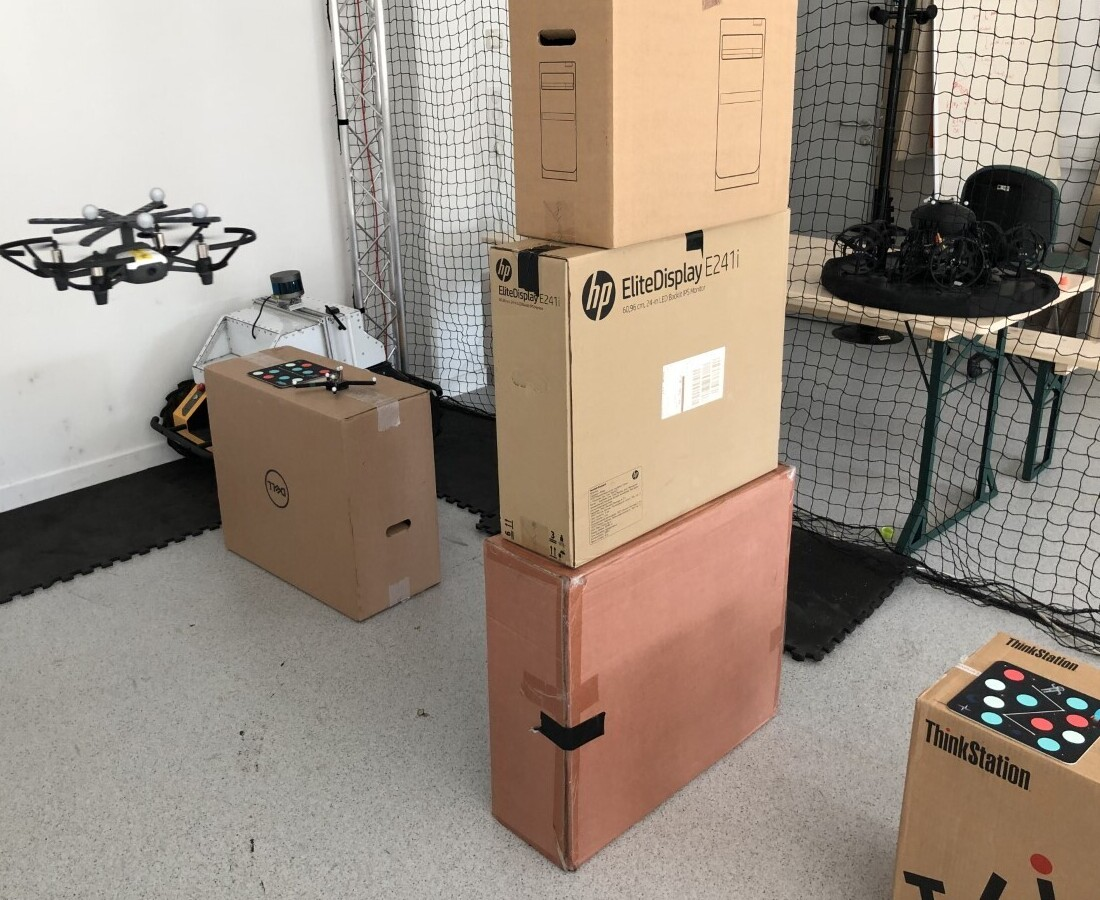
\includegraphics[width=7.2cm]{montage.jpg}
\caption{ \textbf{The flight environment and the drone} }
\label{fig:montage}
\end{figure}

\subsection{The flight environment}
The area in which the drone flies can contain several obstacles. Because of the way it was implemented the obstacles must be rectangular and parallel to the orthogonal directions of the spatial system. In the code, the environment has a set of boundaries and a list of rectangular obstacles, which can be inflated at will. A necessary inflation is to inflate the obstacles with a length equal to the longest diagonal of the drone (121.68 mm), so only a point is needed as a representation of the drone.  The variety of obstacles can obviously be extended, as long as a function verifying potential collisions between a trajectory and the new type of obstacle exists. The area also contains several infrared sensors which can detect the drone with an accuracy down to around 2 mm, and with a detecting rate up to a 100Hz. The control frequency of the drone is thus chosen accordingly, at around 100 Hz as well. As the drone is placed in a closed environment, the installation of infrared sensors was natural. However, the monitoring of a system could be extended to outdoor complex systems, for instance with an interval observer using the available sensors~\cite{Quadrotors Observer,observer}.

\section{PATH PLANNING AND COMMAND OF THE DRONE}
In this section, the path planning of the drone will be discussed. It is important to differentiate the global path planner, used to find a list of way points from the starting position of the drone to the destination, and the local command which generates the right commands so the drone can successively attain all the way points.
\subsection{Path planning} 
The path is determined by using an algorithm, which was strongly inspired by the Rapidly-exploring Random Trees \textit{RRT} and its upgraded version \textit{RRT*}~\cite{RRT,3D_RRT} . The main difference between the implemented versions and the original ones lies in the fact that the dynamic model is not taken into account for the local planning motion. In the case of the drone, this approximation can be justified as the drone can locally move in all the directions in space without much constraints, unlike a car which requires a lot more manoeuvres to park for instance. The drone is a holonomic system.

\begin{figure}[h!]
\centering
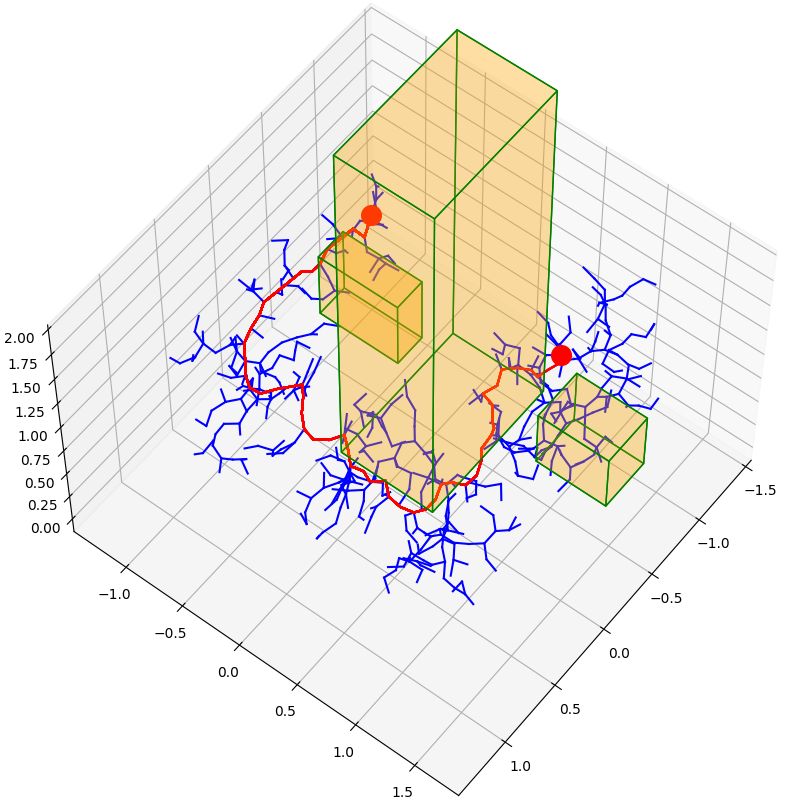
\includegraphics[width=7.8cm]{rrt.png}
\caption{ \textbf{Expanding tree using \textit{RRT} algorithm} between a starting point and a destination, with 3 obstacles in the scene}
\label{fig:image1}
\end{figure}

\begin{algorithm}
 \caption{RRT \cite{RRT}}\label{alg:RRT}
 \begin{algorithmic}[1]
\State $V \gets \{x_{init}\}$; $E \gets \emptyset$; 
\For{$i\gets 1,n$}
    \State $x_{rand} \gets SampleFree_{i};$
    \State $x_{nearest} \gets Nearest(G = (V,E), x_{rand});$
    \State $x_{new} \gets Steer(x_{nearest}, x_{rand});$
    \If{$ObstacleFree(x_{nearest}, x_{new})$}
        \State $V \gets V \cup \{x_{new}\}; E \gets E \cup \{ (x_{nearest}, x_{new}) \}$;
    \EndIf
\EndFor
\State \Return $G=(V,E);$
\end{algorithmic}
\end{algorithm}


The principle of the RRT (\textbf{Algorithm} \ref{alg:RRT}~\cite{RRT}) is to generate an expanding tree of way points from a root (the starting position) with random nodes. The tree keeps expanding until it reaches the destination. At each step, a random position is drawn $x_{rand}$ , then the nearest node belonging to the tree is determined. The new node introduced to the tree $x_{new}$, corresponds to the node at a step distance from $x_{nearest}$ in the direction of $x_{rand}$ and free of collision. The \textit{RRT} was first implemented because it was easier to. However it is proven and can easily be observed even with a relatively high number of iterations that this algorithm is not asymptotically optimal~\cite{RRT}.\\


\begin{algorithm}
 \caption{RRT* \cite{RRT}}\label{alg:RRT2}
 \begin{algorithmic}[1]
\State $V \gets \{x_{init}\}$; $E \gets \emptyset$; 
\For{$i\gets 1,n$}
    \State $x_{rand} \gets SampleFree_{i};$
    \State $x_{nearest} \gets Nearest(G = (V,E), x_{rand});$
    \State $x_{new} \gets Steer(x_{nearest}, x_{rand});$
    \If{$ObstacleFree(x_{nearest}, x_{new})$}
        \State $X_{near} \gets Near(G = (V,E), x_{new}, $
        \State $min \{ \gamma_{RRT*}(log(card(V))/card(V))^{1/d}, \eta \});$
        \State $V \gets V \cap \{x_{new}\};$
        \State $x_{min} \gets x_{init}$; $c_{min} \gets \infty;$
        
        \For{$x_{near} \in X_{near}$} \hspace{1cm}  //First For loop
            \If{$CollisionFree(x_{near},x_{new})$ \& $Cost(x_{near}) +  c(Line(x_{near}, x_{new})) < c_{min} $}
                \State $x_{min} \gets x_{near}$;
                \State $c_{min} \gets Cost(x_{near}) + c(Line(x_{near},x_{new}))$;
            \EndIf
        \EndFor
        \State $E \gets E\cup\{(x_{min},x_{new})\};$ 
        
        \For{$x_{near} \in X_{near}$}\hspace{1cm}  //Second For loop
            \If{$CollisionFree(x_{near},x_{new})$ \& $Cost(x_{new}) +  c(Line(x_{near}, x_{new})) < Cost(x_{near}) $}
                \State $x_{parent} \gets Parent(x_{near});$
                \State $E \gets (E\setminus\{(x_{parent},x_{near}) \cup \{(x_{new},x_{near})\};$
            \EndIf
        \EndFor
    \EndIf
\EndFor
\State \Return $G = (V,E);$
\end{algorithmic}
\end{algorithm}

Let's discuss a few notations from the \textit{RRT*} algorithm (\textbf{Algorithm} \ref{alg:RRT2}~\cite{RRT}) to understand it. In this case, the $Line$ refers to the straight line path between its two arguments. The $Parent : V \rightarrow V$ function returns the parent node of its argument, the parent node of the root being the root itself (or a null pointer to identify it). The $Cost : V \rightarrow \mathbb{R_{+}}$ function returns the cost of the unique path between the argument and the root \cite{RRT} (It measures a distance in our case). The $c$ function returns the distance along a line. $\gamma_{RRT*}$ refers to the search radius of neighbouring nodes,  and $\eta$ refers to the step length between a new node and its parent node.
% The \textit{RRT*} algorithm (\textbf{Algorithm} \ref{alg:RRT2}~\cite{RRT}) works in the same way as the \textit{RRT} algorithm.
The \textbf{Algorithm} \ref{alg:RRT} and the \textbf{Algorithm} \ref{alg:RRT2} begin the same way. However, before inserting a new node $x_{new}$ to the tree, the \textit{RRT*} algorithm finds all the neighbouring nodes in a search radius and determines $x_{new}$'s parent optimizing the cost function (The First For loop of the algorithm). And then, the \textit{RRT*} algorithm considers $x_{new}$ as a potential new parent for its neighbouring nodes, and rewires the tree to optimize the cost function as well (The Second For loop of the algorithm). \textit{RRT*} was proven to be asymptotically optimal, and was thus implemented in the final version.\\

One of the advantage of the \textit{RRT} algorithms is their time complexity which is following an \textit{\textbf{O}}\textit{(nlogn)} complexity in terms of processing, and an \textit{\textbf{O}}\textit{(n)} complexity in terms of queries~\cite{RRT}. There are other variants of the RRT algorithms, for the one implemented in the drone, there is a little bias which chooses directly the destination node, as the `new random` node, at a specified rate. This variant is referred as Artificial Potential Fields (APF)~\cite{3D_RRT}.

\begin{figure}[h]
\centering
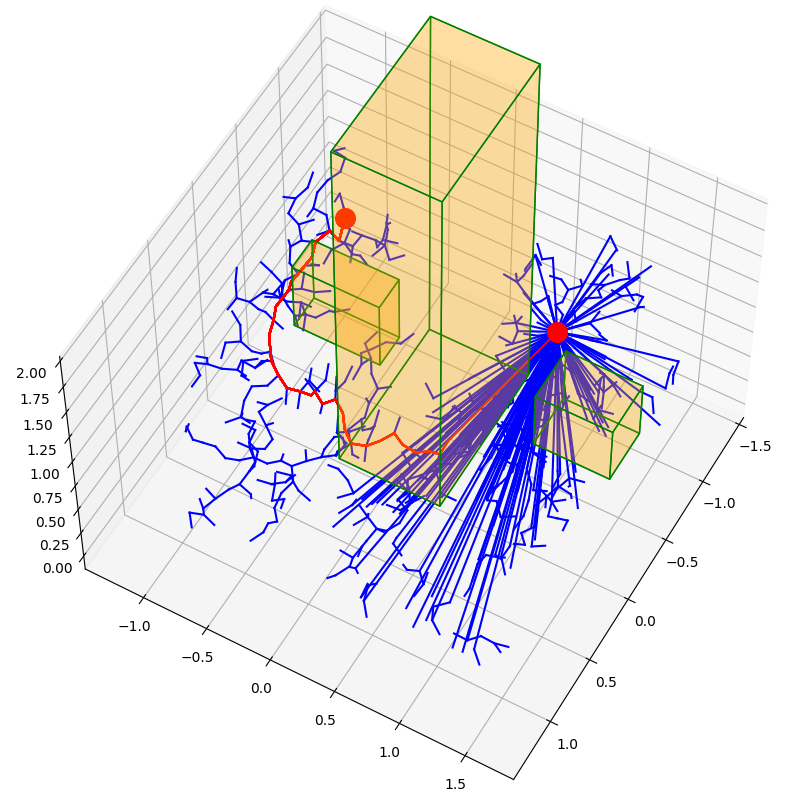
\includegraphics[width=7.8cm]{rrt_star.png}
\caption{ \textbf{Expanding tree using \textit{RRT*} algorithm}}
\label{fig:image2}
\end{figure}


\subsection{Control of the drone}
Thanks to the previous subsection, it is possible to obtain a set of several way points between a starting point and a destination. Since a clear path is planned, with the use of the infrared sensors in the area of flight, it was possible to have a closed loop system. Once again, the monitoring of trajectories could be further extended in cases where an interval observer is required~\cite{Quadrotors Observer}. In the case of an interval observer, the uncertainties linked to the observer would be greater and would need to be considered in our model based on interval analysis. \\

A PI (Proportional Integral) controller was implemented for the drone. This controller came naturally, since the coefficients could have been tuned thanks to interval analysis as well~\cite{PI}. Besides, it is worth mentionning that the \textit{RRT*} algorithm can produce relatively long straight lines, as it rewires and find shortcuts between nodes. In the case of a Proportional controller, the drone could accumulate a lot of inertia even with a saturation. That's why in the case of a long distance between two way points, intermediate points were introduced. Any path folowing algorithms can be used to perform this task, even with wind\cite{pathfol} or for a vision-based control \cite{pathfol2}.\\


Obviously, each geometrical position of the way points cannot be reached perfectly by a drone. A margin was implemented so that a way point can be considered reached more easily. This margin was reduced to a minimum during the landing phase with the purpose of having the most accurate landing possible. Those margins add uncertainties to our model as well.\\

Considering the PI controller, it is possible to define more precisely the commanded inputs:

\begin{equation}
    \left\{
    \begin{array}{ll}
        u_{x} = K_{P} * ( x_{waypoint} - x_{position}(t_{n}) )\\
    \hspace{1cm} + \hspace{0.2cm} K_{I} * \sum_{i=n_{prev}}^{n}( x_{waypoint} - x_{position}(t_{i}))\\
        u_{y} = K_{P} * ( y_{waypoint} - y_{position}(t_{n}) )\\
    \hspace{1cm} + \hspace{0.2cm} K_{I} * \sum_{i=n_{prev}}^{n}( y_{waypoint} - y_{position}(t_{i}))\\
    u_{z} = K_{P} * ( z_{waypoint} - z_{position}(t_{n}) )\\
    \hspace{1cm} + \hspace{0.2cm} K_{I} * \sum_{i=n_{prev}}^{n}( z_{waypoint} - z_{position}(t_{i}))\\
    \end{array}
    \right.
\end{equation}\\
where $n$ corresponds to the current index of time, and $n_{prev}$ the previous index of time upon reaching the previous way point.


It is necessary to note that the coefficients $K_{P}$ and $K_{I}$ have a unit in $s^{-1}$. Even with the accuracy of the sensors (around 2mm) and the PI controller, the drone will never perfectly follow the path defined globally, there will always be uncertainties. 


\section{APPLIED INTERVAL ANALYSIS AND OUR MODEL}

\subsection{A small introduction to interval analysis}

The main underlying tool, used in our design methodology, is
\emph{interval analysis}~\cite{Moore66}. 
There is a need to clarify some notations that will be reccurently used. The following notation $\lbrack x \rbrack \in \mathbb{IR}$ represents an interval $\lbrack x \rbrack =
\lbrack\underline{x}, \overline{x}\rbrack=\{ x \in \Rset \mid
\underline{x} \leqslant x \leqslant \overline{x} \}$. And $\mathbb{IR}$ is the set of
intervals with real bounds. By abuse of notation, $[x]$ will also denote a vector of
intervals, \emph{i.e.}, a Cartesian product of intervals, a.k.a. a
\emph{box}. In our case, the boxes will obviously be three dimensionnals.\\

In this article, interval analysis is meant to take into account all the uncertainties. So the uncertainties will be considered as uniform distributions. Indeed, a uniform distribution allows to encompass even the worst possible cases~\cite{Reliabilty}.
Without going in depth, the notions of contractors and solvers will also implicitely be used in the next section~\cite{Jaulin}.

\subsection{Establishing our model based on the control}
Thanks to the path planning section, and more particularly the local command in speed, a rather simplistic model of the drone behaviour was established:
\begin{equation}
    \left\{
    \begin{array}{ll}
        \dot{x} = u_{x} \\
        \dot{y} = u_{y} \\
        \dot{z} = u_{z}
    \end{array}
    \textit{or } \dot{\textbf{w}} = \textbf{u}
    \right.
\end{equation}
The command $\textbf{u}$ was detailled in the previous section as well.\\
The infrared sensors allow the user to have the position of the drone at a given time. Thus, it is an interval initial value problem, with an ordinary differential equation in the following form.

\begin{equation}
    \dot{y} = f(y) \text{ with } y(0) \in \lbrack y_{0} \rbrack \text{ and } t \in \lbrack 0,t_{horizon} \rbrack
\end{equation}

It is assumed that the function $f : \mathbb{R}^{3} \rightarrow \mathbb{R}^{3}$ is globally Lipschitz in $y$, and here corresponds to the flow. $y$ would be the position of the drone, and $[y_{0}]$ corresponds to the uncertainty due to the sensors' accuracy. $t_{horizon}$ will be more detailed in a latter section, but it reprensents the time during which each simulation is made~ \cite{Sandretto}.\\

An arsenal of validated Runge-Kutta methods exists to compute the sets of boxes, solution to these types of ordinary differential equation~\cite{Sandretto}. A little reminder of what a validated numerical integration does at each step~\cite{Sandretto}:\vspace{0.2cm}\\ 
\textbf{Phase 1  } One computes an \textit{a priori} enclosure $\lbrack \tilde{y_{j}} \rbrack$ of the solution such that
\begin{itemize}
  \item $y(t;\lbrack y_{j} \rbrack)$ is guaranteed to exist for all $t \in \lbrack t_{j}, t_{j+1} \rbrack$, \textit{i.e} along the current step, and for all $y_{j} \in \lbrack y_{j} \rbrack$ \vspace{0.2 cm}
  \item $y(t; \lbrack y_{j} \rbrack ) \subseteq \lbrack \tilde{y_{j}} \rbrack$ for all $t \in \lbrack t_{j}, t_{j+1} \rbrack$ \vspace{0.2cm}
  \item the step-size $h_{j} = t_{j+1} - t_{j} > 0$ is as large as possible in terms of accuracy and existence proof \vspace{0.2 cm}
\end{itemize}
\textbf{Phase 2  } One computes a tighter enclosure of $\lbrack y_{j+1} \rbrack$ at time $t_{j+1}$, such that $y(t_{j+1}, \lbrack y_{j} \rbrack ) \subseteq \lbrack y_{j+1} \rbrack$.\\
%citer l'article sur validated ...

In this article, we have mentionned the presence of several uncertainties which can impact the commanded inputs. That's why, an affine form for the commanded inputs was introduced in the model. An affine form provides a simple model which helps to have faster computation times for the monitoring, and encompasses largely the uncertainties.
\begin{equation}
    \left\{
    \begin{array}{ll}
        \dot{x} = \lbrack \alpha_{x} \rbrack * u_{x} + \lbrack \beta_{x} \rbrack  \\
        \dot{y} = \lbrack \alpha_{y} \rbrack * u_{y} + \lbrack \beta_{y} \rbrack  \\
        \dot{z} = \lbrack \alpha_{z} \rbrack * u_{z} + \lbrack \beta_{z} \rbrack
    \end{array}
    \textit{or } \dot{\textbf{w}} = \lbrack \alpha \rbrack * \textbf{u} + \lbrack \beta \rbrack
    \right.
\end{equation}

A model established with this form is a way to consider a large panel of uncertainties.\\
\textbf{The presence of $\lbrack \alpha \rbrack$:}
\begin{itemize}
  \item corrects the assumption of immediate commanded inputs and includes the drone's speed profile\vspace{0.2cm}
  \item  takes into account all uncertainties linked to forces which have dependecies with the velocity\vspace{0.2cm}
  \item takes into consideration uncertainties linked to the tuning of the coefficients $K_{P}$ and $K_{I}$~\cite{PI}
\end{itemize}

\textbf{The presence of $\lbrack \beta \rbrack$:}
\begin{itemize}
  \item corrects all uncertainties linked to punctual pertubations\vspace{0.2cm}
  \item considers ambient noises in the command and induced by the drone itself \vspace{0.2cm}
\end{itemize}

Let's introduce scores of how well the model was built when the various uncertainties were considered. It is possible to introduce a coefficient $c_{\cup}$ measuring the number of times the computed boxes were intersecting with the trajectory, and another coefficient $c_{\subset}$ measuring the number of times the trajectory was actually included in the computed boxes. In this case, the trajectory are boxes with the length of the sensors' uncertainty.
\begin{equation}
    \left\{
    \begin{array}{ll}
        c_{\cap} = \frac{\text{Number of intersections}}{\text{Total number of comparisons}} \\
        c_{\subset} = \frac{\text{Number of inclusions}}{\text{Total number of comparisons}}
    \end{array}
    \right.
\end{equation}
The interval coefficients $\lbrack \alpha \rbrack$ and $\lbrack \beta \rbrack$ were determined for a collision free trajectory, and based on optimizing these two scores:
\begin{equation}
    \left\{
    \lbrack \alpha \rbrack * \textbf{u} + \lbrack \beta \rbrack = 
    \begin{pmatrix}
        \lbrack 0, 1 \rbrack \\
        \lbrack -0.4, 0.4 \rbrack \\
        \lbrack -0.4, 0.4 \rbrack \\
    \end{pmatrix}
    * \textbf{u} +
    \begin{pmatrix}
        \lbrack -0.1, 0.1 \rbrack \\
        \lbrack -0.1, 0.1 \rbrack \\
        \lbrack -0.1, 0.1 \rbrack \\
    \end{pmatrix}
    \right.
\end{equation}
\vspace{0.1cm}
\section{MONITORING OUR TRAJECTORY WITH DYNIBEX}

\subsection{Principle of the monitoring}
Now that a model has been established, it will be possible to compute a set of boxes representing the drone's behaviour. The trajectory of the drone should be inside those boxes. Those boxes will be computed thanks to the library DynIbex. Indeed, DynIbex will be used to resolve the equations representing our model. DynIbex uses the theory of applied interval analysis, and affine arithmetic to solve various types of differential equations. In this case, the differential equation is rather simple, but DynIbex allows a relatively fast and validated integration. The Runge-Kutta method used in this article is Heun's method. With the help of the computed boxes, it will be possible to monitor the trajectory of the drone. Indeed since our obstacles are rectangular and in the same directions as the spatial system, they can easily be converted to boxes. DynIbex has a feature that allows us to check if boxes intersect or are subsets of each other. If we were to later introduce more complex obstacles, an interesting solution would be to decompose the complex obstacles into several rectangular obstacles.\\

The principle of the monitoring is then easier to implement. As the drone determines its trajectory, DynIbex will compute whether or not the drone will be within a set of boxes, guaranteed to reach the way points, and not collide with any of the obstacles. A similar work has been done, but the idea was not to monitor the trajectory with DyniBEX, but directly compute the trajectory of a system as a set of boxes, using an RRT algorithm~\cite{box_RRT}. The issue with this method in our case, is that the computed boxes would rapidly diverge unless the model was more accurate. Besides, it is likely that building an RRT tree, with boxes as nodes in a 3D space, might take a long time.\\

In terms of implementation, if the trajectory determined by the global planner were monitored by our solver and deemed incorrect because of a potential collision, the idea would be to inflate even more the obstacles with the purpose of adding a margin of security against collisions. So far, the monitoring is done, \emph{a posteriori}, over the course of the whole trajectory. But with a little bit more time and implementation, it would be possible to imagine a real-time monitoring, the trajectory would be monitored continuously over a sliding horizon of time~\cite{Sliding}. The monitoring would be focused on detecting potential collisions, induced by moving obstacles or by an innacurate trajectory, and would launch the planning of a new trajectory.

\subsection{Observations and Results} 
In the previous section, a $t_{horizon}$ was mentionned, this $t_{horizon}$ represents the time during which each computation of the boxes should be made, before another measure of position is detected. Depending on this $t_{horizon}$, our model will have to be more refined with its uncertainties ($\lbrack \alpha \rbrack$ and $\lbrack \beta \rbrack$). Let's dicuss it with examples:
\begin{figure}[h!]
\centering
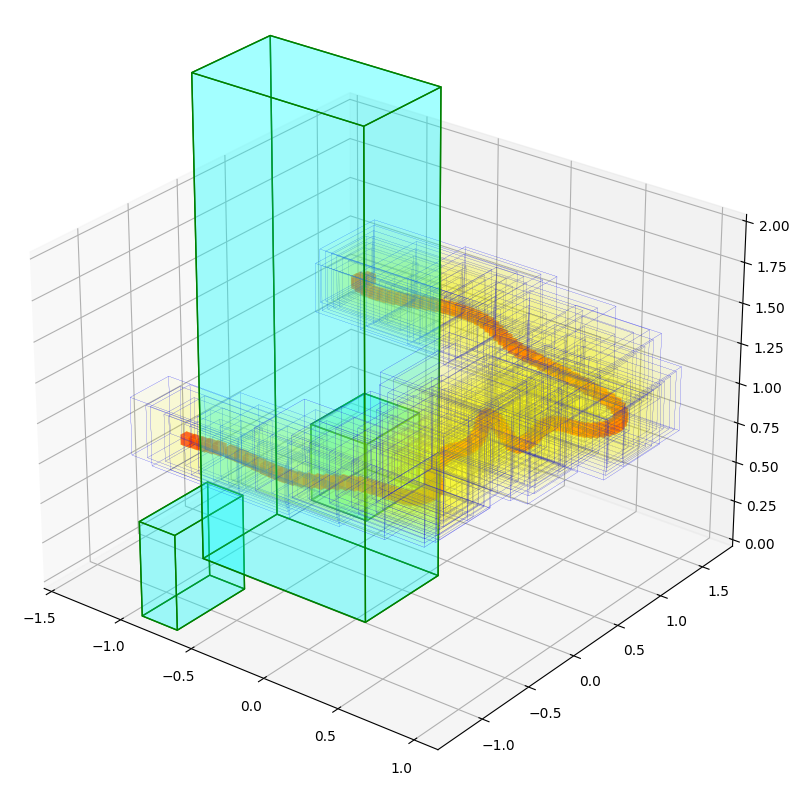
\includegraphics[width=7.8cm]{dynibex.png}
\caption{ \textbf{In yellow the computed boxes for $t_{horizon} = 1 s$ with the adjusted $\lbrack \alpha \rbrack$ and $\lbrack \beta \rbrack$ (Collision free), in red the actual trajectory followed by the drone}}
\label{fig:image3}
\end{figure}

\begin{figure}[h!]
\centering
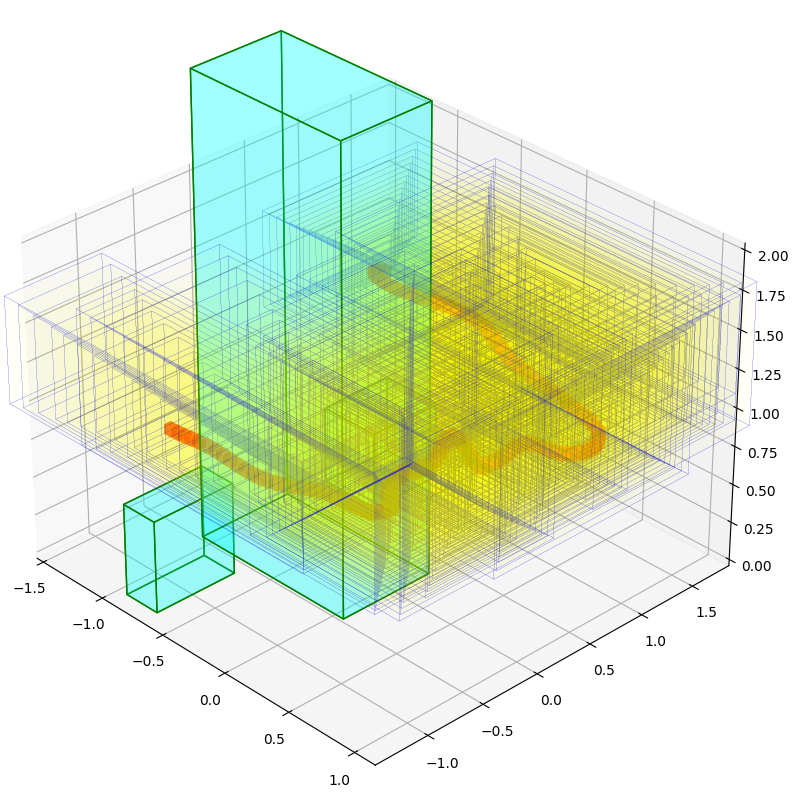
\includegraphics[width=7.8cm]{dynibex_3s.png}
\caption{ \textbf{In yellow the computed boxes for $t_{horizon} = 3 $ s with the adjusted uncertainties for $t_{horizon} = 1 s$  (Collision), in red the actual trajectory followed by the drone}}
\label{fig:image4}
\end{figure}
As it is visually observable in Figure \ref{fig:image3} and Figure \ref{fig:image4}, when the uncertainties considered for $t_{horizon} = 1 $ s were kept for a computation with $t_{horizon} = 3 $ s, the computed boxes started to diverge. Indeed, the uncertainties considered were too rough, and since the computation time is greater, the computed boxes have the time to accumulate the uncertainties until this horizon of time. If we were to monitor this trajectory beforehand, we would definitively not let the drone fly as the computed boxes would detect a collision with the obstacles.\\

However, since the model was built too simplistically, it is difficult to refine the uncertainties so that it could perfectly coincide with the reality and have a $t_{horizon}$ tending toward infinity. 

\begin{figure}[h!]
\centering
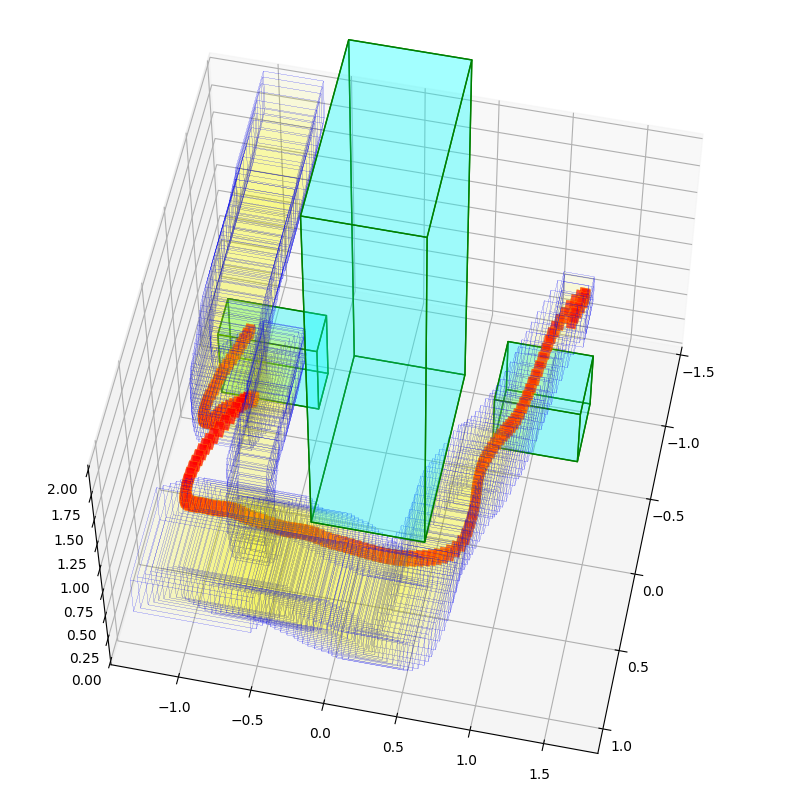
\includegraphics[width=7.8cm]{dynibex_15s.png}
\caption{ \textbf{In yellow the computed boxes for $t_{horizon} = 15$ s with the adjusted uncertainties for $t_{horizon} = 1$ s, in red the actual trajectory followed by the drone}}
\label{fig:dynibex_15s}
\end{figure}

As it can be seen in the Figure \ref{fig:dynibex_15s}, although the computed boxes follow correctly the trajectory in the beginning, when the horizon of time is too far ahead, the simulation still starts to diverge and does not encapsulate the trajectory properly. Actually, the simulated trajectory is closed to how the drone would fly if it were in an open-loop control. Near the end of the trajectory, there are several tubes of computed boxes. As the flight lasted longer than $15 s$, the several simulations happened to be visible. The effect is not in the Figures \ref{fig:image3} and \ref{fig:image4}, because the various tubes overlap as their horizons of time are short.

There is a strong link between the creation of the model and the efficiency of the method. The scores using the adjusted interval coefficients $\lbrack \alpha \rbrack$ and $\lbrack \beta \rbrack$ for $t_{horizon} = 1$ s, with the following $t_{horizon}$, is a reflect of this link.\\

\begin{tabular}{ |p{1.5cm}||p{1.2cm}|p{1.2cm}|p{1.2cm}|p{1.2cm}| }
 \hline
 \multicolumn{5}{|c|}{Scores and collision} \\
 \hline
 $t_{horizon}$ & 1 s  & 3 s & 12s & 15 s \\
 \hline
 $c_{\cap}$    & 1    & 1   & 1   & 0.786\\
 \hline
 $c_{\subset}$ & 0.687 & 0.676 & 0.899 &0.59\\
 \hline
collision ? & No & Yes & Yes & Yes\\
 \hline
\end{tabular}\\

\vspace{0.2 cm}Naturally as $t_{horizon}$ increases, the uncertainties have more time to diverge (get bigger), and the scores $c_{\cap}$ and $c_{\subset}$ increase as they encompass a large part of the arena. However, the scores could also decrease for specific $t_{horizon}$, as the simulation would completely go off course in time. In the end, it is essential to tune the interval coefficients ($\lbrack \alpha \rbrack$ and $\lbrack \beta \rbrack$) and the security margins while ensuring a collision free trajectory, using the scores $c_{\cap}$ and $c_{\subset}$, but also while considering the right horizon of time depending on the system. 


\section{CONCLUSIONS}
The paper introduced a method to monitor trajectories using interval analysis. The method is based on balancing several aspects of the model. Indeed, for the method to work efficiently, there is a need to have a balance between the accuracy of the model, the uncertainties linked to the sensors and the observer, the inherent uncertainties induced by the system and the horizon of computation time. After finding the balance between all those criteria, the method will allow to determine the reliability of trajectories. As mentionned in the introduction, there is room for improvements on several aspects, and a case study with a more complex model and greater  uncertainties could better demonstrate the efficiency of the method. 



\addtolength{\textheight}{-12cm}   % This command serves to balance the column lengths
                                  % on the last page of the document manually. It shortens
                                  % the textheight of the last page by a suitable amount.
                                  % This command does not take effect until the next page
                                  % so it should come on the page before the last. Make
                                  % sure that you do not shorten the textheight too much.

%%%%%%%%%%%%%%%%%%%%%%%%%%%%%%%%%%%%%%%%%%%%%%%%%%%%%%%%%%%%%%%%%%%%%%%%%%%%%%%%



%%%%%%%%%%%%%%%%%%%%%%%%%%%%%%%%%%%%%%%%%%%%%%%%%%%%%%%%%%%%%%%%%%%%%%%%%%%%%%%%



%%%%%%%%%%%%%%%%%%%%%%%%%%%%%%%%%%%%%%%%%%%%%%%%%%%%%%%%%%%%%%%%%%%%%%%%%%%%%%%%
% \section*{APPENDIX}
% 
% Je vais avoir besoin d'aide
% 
% J: pas nécessaire
% 
% \section*{ACKNOWLEDGMENT}
% 
% Je vais avoir besoind d'aide
% 
% J: aucun financement particulier, on mettra peut être le projet DGA FARO.


%%%%%%%%%%%%%%%%%%%%%%%%%%%%%%%%%%%%%%%%%%%%%%%%%%%%%%%%%%%%%%%%%%%%%%%%%%%%%%%%


\begin{thebibliography}{99}

%\bibitem{Moore} Traub, J. F. (1967). Assessing Accuracy: Interval Analysis. Ramon E. Moore. Prentice-Hall, Englewood Cliffs, NJ, 1966. 159 pp., illus. \$9. Science, 158(3799), 365-365.

\bibitem{Moore66} Moore, Ramon (1966). Interval Analysis. Prentice Hall, 1966. %Plutot celui ci

\bibitem{Jaulin} Jaulin, L., Kieffer, M., Didrit, O., \& Walter, E. Applied interval analysis, 2001. ed: Springer, London.

\bibitem{Sandretto} Alexandre dit Sandretto, J., \& Chapoutot, A. (2016). Validated explicit and implicit Runge-Kutta methods. Reliable Computing electronic edition, 22.

\bibitem{Guaranteed}Rohou, S., Jaulin, L., Mihaylova, L., Le Bars, F., \& Veres, S. M. (2017). Guaranteed computation of robot trajectories. Robotics and Autonomous Systems, 93, 76-84.

\bibitem{Reliabilty}Merlet, J. P. (2006). Interval analysis and reliability in robotics.

\bibitem{Quadrotors Observer}Abadi, A., El Amraoui, A., Mekki, H., \& Ramdani, N. (2020). Guaranteed trajectory tracking control based on interval observer for quadrotors. International Journal of Control, 93(11), 2743-2759.

\bibitem{Safe} Kousik, S., Holmes, P., \& Vasudevan, R. (2019). Technical Report: Safe, Aggressive Quadrotor Flight via Reachability-based Trajectory Design. arXiv preprint arXiv:1904.05728.

\bibitem{Robust} Pepy, R., Kieffer, M., \& Walter, E. (2009). Reliable robust path planning. International Journal of Applied Mathematics and Computer Science, 19(3), 413-424.

\bibitem{RRT} Karaman, S., \& Frazzoli, E. (2011). Sampling-based algorithms for optimal motion planning. The international journal of robotics research, 30(7), 846-894.

\bibitem{3D_RRT}Pharpatara, P., Hérissé, B., \& Bestaoui, Y. (2016). 3-D trajectory planning of aerial vehicles using RRT. IEEE Transactions on Control Systems Technology, 25(3), 1116-1123.

\bibitem{observer}Thabet, R. E. H., Raissi, T., Combastel, C., Efimov, D., \& Zolghadri, A. (2014). An effective method to interval observer design for time-varying systems. Automatica, 50(10), 2677-2684.

\bibitem{box_RRT}Panchea, A. M., Chapoutot, A., \& Filliat, D. (2017, December). Extended reliable robust motion planners. In 2017 IEEE 56th Annual Conference on Decision and Control (CDC) (pp. 1112-1117). IEEE

\bibitem{PI} Alexandre dit Sandretto, J., Chapoutot, A., \& Mullier, O. (2015, November). Tuning PI controller in non-linear uncertain closed-loop systems with interval analysis. In 2nd International Workshop on Synthesis of Complex Parameters, OpenAccess Series in Informatics (Vol. 44, pp. 91-102).

\bibitem{Hybrid}Frazzoli, E. (2001). Robust hybrid control for autonomous vehicle motion planning (Doctoral dissertation, Massachusetts Institute of Technology).

\bibitem{Markov}Burlet, J., Aycard, O., \& Fraichard, T. (2004, April). Robust motion planning using markov decision processes and quadtree decomposition. In IEEE International Conference on Robotics and Automation, 2004. Proceedings. ICRA'04. 2004 (Vol. 3, pp. 2820-2825). IEEE

\bibitem{Signal}Lindemann, L., Pappas, G. J., \& Dimarogonas, D. V. (2021). Reactive and risk-aware control for signal temporal logic. IEEE Transactions on Automatic Control.

\bibitem{Sliding}Alexandre dit Sandretto, J., Brendel, E., \& Chapoutot, A. (2018). An Interval-based Sliding Horizon Motion Planning Method. IFAC-PapersOnLine, 51(16), 296-301

\bibitem{pathfol} Mcgee, T. G. et Hedrick, J. K.. Path planning and control for multiple point surveillance by an unmanned aircraft in wind. In : 2006 American Control Conference. IEEE, 2006. p. 6 pp.

\bibitem{pathfol2} Courbon, J., Mezouar, Y., Guénard, N., \& Martinet, P. (2010). Vision-based navigation of unmanned aerial vehicles. Control Engineering Practice, 18(7), 789-799.

\end{thebibliography}




\end{document}
